\documentclass[11pt]{article}
\usepackage[utf8]{inputenc}
\usepackage[T1]{fontenc}
\usepackage[sc]{mathpazo}
\linespread{1.04}
\usepackage[letterpaper,textwidth=6.3in,textheight=8.9in]{geometry}
\usepackage{booktabs}
\usepackage{tabularx}
\usepackage{caption}
\captionsetup{font=small,labelfont=bf,skip=4pt}
\usepackage{url}
\usepackage[hidelinks]{hyperref}
\usepackage{amsmath}
\usepackage{tikz}
\usetikzlibrary{arrows.meta,positioning,calc,shapes.misc}
\usepackage{pgfplots}
\pgfplotsset{compat=1.18}
\tikzset{
  tbl/.style={draw,rectangle,thin,inner sep=5pt,align=left,font=\small,fill=white},
  tblname/.style={font=\small\bfseries},
  box/.style={draw,rectangle,thin,inner sep=4pt,align=center,font=\footnotesize,fill=white,text width=3.0cm},
  wide/.style={box,text width=5.4cm},
  arr/.style={-{Stealth[length=5pt]},thin},
  lab/.style={font=\scriptsize,fill=white,inner sep=1pt}
}
\setlength{\parskip}{0pt}
\sloppy

\newcolumntype{Y}{>{\raggedright\arraybackslash}X}

\title{\large\bfseries Checkpoint 1: Understanding the Dataset and Study Design\\[4pt]
\normalsize\mdseries Conflicting and competing agent skills in the GitSkills dataset}
\author{\normalsize Chris Reger \and \normalsize Smirthya Somaskantha Iyer}
\date{\normalsize CS 599, Northern Arizona University \\ October 22, 2026}

\begin{document}
\maketitle

\noindent Repository: \url{https://github.com/Naalu/agent-skill-conflicts}
\medskip

\noindent Coding agents such as Claude Code, Codex and Cursor can be extended with ``skills,'' small instruction files that
each carry a name and a short description. When the user asks for something, the agent reads the list of names and
descriptions and decides which skill, if any, to load. Our project is about what happens when that list has problems in it:
the same skill copied into several agent folders and then edited separately, so Claude Code and Codex read different
instructions under one name, or two differently named skills whose descriptions overlap so much that we could not say which
one the agent should pick. We want to measure how common each of these is across the 282{,}200 repositories in GitSkills,
and whether skill authors do anything to prevent it.

\section{Dataset overview and available resources}

\subsection{Identification}
The dataset is GitSkills \cite{destefanis2026gitskills}. We work from the Parquet export on Hugging Face
(\texttt{mvaccargiu/gitskills}): the \texttt{artifacts} table is split into 31 files of around 200\,MB, and the other three
tables (\texttt{repos}, \texttt{artifact\_siblings}, \texttt{mining\_runs}) are one file each. The paper also distributes a
single SQLite database on Zenodo (DOI 10.5281/\allowbreak zenodo.21875637). We assumed at first that we would need that one,
but the Parquet files were much easier to process one at a time on a laptop with 16\,GB of memory, so we never downloaded
it. We read the documentation on October 6 and downloaded the files over October 6 to 8 during the pilot work.

The available resources are the dataset paper (arXiv:2608.10906; version 3 is dated September 11, 2026), the Hugging Face
data card, where the download links are, and a small sample repository at
\url{https://github.com/giuseppedestefanis/gitskills-sample}. There is no separate data dictionary; each table gets a paragraph
describing its columns in general terms, and for a couple of columns we worked out the meaning from the values (Section 2).
We found no published notebooks. We read each Parquet part with DuckDB, keep only the columns we need, and delete the part,
which brings the roughly 6\,GB download down to about 300\,MB on disk.

\subsection{Creators and purpose}
GitSkills was created by Giuseppe Destefanis (University College London), Daniel Graziotin and Matteo Vaccargiu (University
of Hohenheim), and Marco Ortu (University of Cagliari) for the MSR 2027 Mining Challenge \cite{msr2027call}. The paper says it
is meant to support research on how skills are adopted, reused, structured, written, maintained and secured; our study sits
at the reuse and maintenance end of that list.

\subsection{Sources, collection period, inclusion and exclusion}
All of the data comes from public GitHub repositories. The authors used GitHub code search to find files named
\texttt{SKILL.md}, downloaded the text from GitHub's raw-content CDN, and pulled repository metadata and commit history from
the REST API.

For the collection period the \texttt{mining\_runs} table was more useful than the paper. It lists seven runs between July 9,
2026 (17:26 UTC) and July 20, 2026 (22:26 UTC). Two runs did almost all of the work, discovering 1{,}328{,}473 and
1{,}657{,}948 files; the other four carry the note ``closed retroactively: process crashed before finishing.'' Our first
pilot used July 31 as the snapshot date, because that is what ``July 2026'' in the paper suggested to us; only when we opened
\texttt{mining\_runs} did we see that the last run ended on July 20. That mattered for the retired-model pilot mentioned in
Section 6, where seventeen OpenAI models retired on July 23 had been counted as already retired at collection, and moving
the date brought one headline figure from 36.0\% down to 32.8\%.

The only inclusion rule the authors applied is the file name. Everything else is a limit of GitHub code search, which
indexes only the default branch, only files under 384\,KB, only repositories with fewer than 500{,}000 files and some recent
activity, and forks only when the fork has more stars than the original. The 1{,}000-result cap per query was worked around
by splitting the search by file size. Every occurrence is kept with its repository, path and content hash; the text, front
matter and commit history are stored once per distinct content, on the copy marked as representative
(\texttt{dedup\_primary = 1}).

\subsection{Artifacts, coverage and counts}
\begin{table}[h]
\centering\small
\begin{tabular}{lrl}
\toprule
Table & Rows & One row is \\
\midrule
\texttt{artifacts} & 3{,}797{,}117 & one \texttt{SKILL.md} file occurrence (repository plus path) \\
\texttt{artifact\_siblings} & 7{,}264{,}865 & one file or directory beside a representative skill \\
\texttt{repos} & 282{,}200 & one repository \\
\texttt{mining\_runs} & 7 & one search run \\
\bottomrule
\end{tabular}
\caption{The four tables. Row counts are from the data card; we checked them against the Parquet files on October 8.}
\end{table}

The 3{,}797{,}117 occurrences collapse to 1{,}877{,}981 distinct contents, so just over half of the rows (50.5\%) are
byte-for-byte copies of a file that also exists somewhere else. 3{,}742{,}828 rows (98.6\%) are named exactly
\texttt{SKILL.md}; the rest differ in capitalization or carry a suffix. The front matter parses and contains both a name and a
description for 3{,}385{,}119 occurrences (89.2\%), or 1{,}612{,}967 distinct contents. Commit history exists for 458{,}548
representative copies, 24.4\% of distinct contents. The authors' \texttt{location\_class} column puts 2{,}102{,}053 rows in
\texttt{skills-dir}, 1{,}321{,}412 in \texttt{other} and 373{,}652 in \texttt{canonical}. The median repository has zero stars
(mean 122), only three repositories are flagged as forks, and 156{,}466 (55\%) have an empty license field.

\subsection{License}
The metadata and the aggregation are released under CC-BY-4.0. The \texttt{content} column reproduces text from other
people's repositories, which stays under the original repository's license (\texttt{repos.license}). Since more than half of
the repositories declare no license, we will not redistribute skill text in bulk; our replication package will hold
aggregates, our labels and pseudonymous identifiers.

The authors replaced commit author accounts with keyed one-way codes and redacted e-mail addresses and personal names in
commit messages, leaving in the names of AI assistants in \texttt{Co-authored-by} trailers. The challenge rules add that
``The share or use of personally identifiable information (PII) is strictly prohibited'' \cite{msr2027call}, which we treat
as applying to our repository as well as to the paper.

\subsection{Collection period versus artifact dates}
The snapshot is from July 2026, but the files in it were written over the preceding year. Of the 458{,}137 representative
copies with a first-commit date, 152 are from before October 2025, earlier than the skill format existed, presumably files
later turned into skills or that happened to share the name. After that the monthly counts grow quickly:
1{,}265 in October 2025, 3{,}578 in November, 6{,}615 in December, 20{,}918 in January 2026, 49{,}234 in February, 78{,}540
in March, 84{,}062 in April, 86{,}254 in May, 85{,}855 in June, and 41{,}664 in the twenty days of July that were covered
(Figure~\ref{fig:months}).

\begin{figure}[h]
\centering
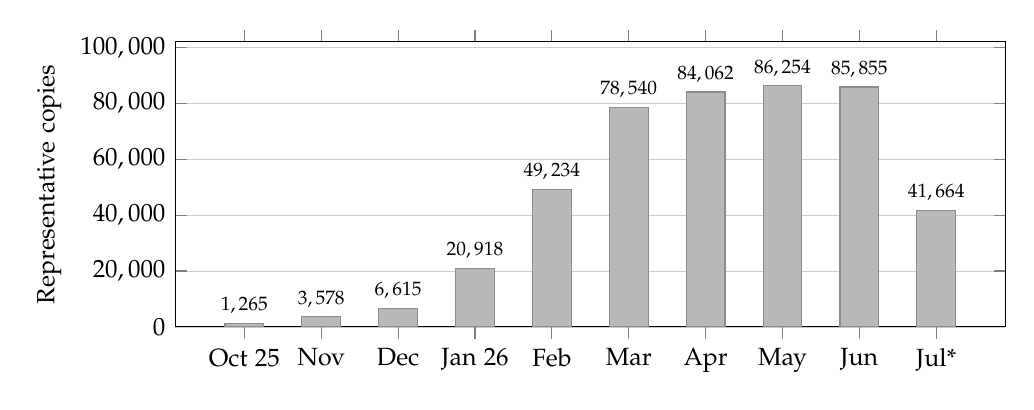
\begin{tikzpicture}
\begin{axis}[
  width=\textwidth, height=5.2cm, ybar, bar width=14pt,
  ymin=0, ymax=102000,
  ylabel={Representative copies}, ylabel style={font=\small},
  symbolic x coords={Oct 25,Nov,Dec,Jan 26,Feb,Mar,Apr,May,Jun,Jul*},
  xtick=data, x tick label style={font=\small}, y tick label style={font=\small},
  scaled y ticks=false,   nodes near coords, nodes near coords style={font=\scriptsize},
  axis line style={thin}, tick style={thin}, ymajorgrids, grid style={very thin,gray!40},
  /pgf/number format/.cd, fixed, 1000 sep={,},
]
\addplot[fill=gray!55, draw=gray!90] coordinates {(Oct 25,1265) (Nov,3578) (Dec,6615) (Jan 26,20918) (Feb,49234) (Mar,78540) (Apr,84062) (May,86254) (Jun,85855) (Jul*,41664)};
\end{axis}
\end{tikzpicture}
\caption{First-commit month of the 458{,}137 representative copies that have a commit date. The 152 copies dated before October 2025 are left out. *July covers only the twenty days up to the last mining run.}
\label{fig:months}
\end{figure}

Any trend we plot therefore stops abruptly in July 2026, and the age of a skill has to be computed from its first commit to
July 20, 2026, not to the day we run the analysis; star counts and \texttt{pushed\_at} dates are likewise as of the July
fetch. We also realized only after the retired-model pilot that the copy carrying the history is the representative, not the
oldest copy (on a sample of content hashes with several dated copies, the representative was the earliest in well under
half), so the first-commit date we have is a lower bound on the age of the content.

\subsection{What the dataset does not capture}
What worries us most is what sits outside repositories. When Claude Code builds its list of skills it includes the user's
personal skills, skills that came with installed plugins, and a few that ship with the product, and none of that is in
GitSkills because none of it is committed to a project repository. Whatever prevalence we report will understate what an
agent sees in practice, possibly by a lot for heavy users of plugins, and we cannot estimate that gap from this data.

Smaller gaps: non-default branches are not indexed, skills deleted or renamed before July are gone, and any repository the
search did not return is simply absent. The dataset says nothing about whether a skill was ever loaded, by which agent, or
what the agent did afterwards. Commit history is missing for three quarters of distinct contents, and nothing says which
copy of a shared content came first. Forks are almost entirely absent, so copying between a fork and its parent is
invisible, though copying between unrelated repositories shows up through the shared hash.

\section{Data structure and relationships}

\begin{figure}[h]
\centering
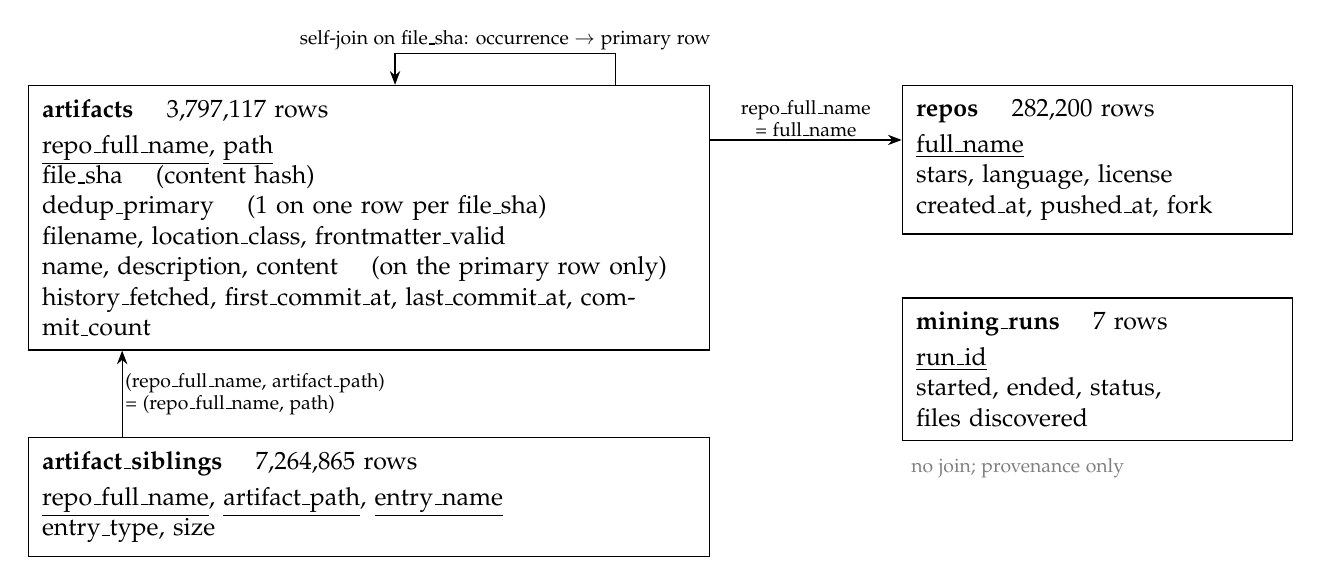
\begin{tikzpicture}
\node[tbl,text width=8.3cm,anchor=north west] (art) at (0,0) {\textbf{artifacts} \quad 3{,}797{,}117 rows\\[2pt]
  \underline{repo\_full\_name}, \underline{path}\\
  file\_sha \quad (content hash)\\
  dedup\_primary \quad (1 on one row per file\_sha)\\
  filename, location\_class, frontmatter\_valid\\
  name, description, content \quad (on the primary row only)\\
  history\_fetched, first\_commit\_at, last\_commit\_at, commit\_count};
\node[tbl,text width=4.6cm,anchor=north west] (repos) at (11.1,0) {\textbf{repos} \quad 282{,}200 rows\\[2pt]
  \underline{full\_name}\\
  stars, language, license\\
  created\_at, pushed\_at, fork};
\node[tbl,text width=4.6cm,anchor=north west] (runs) at (11.1,-2.7) {\textbf{mining\_runs} \quad 7 rows\\[2pt]
  \underline{run\_id}\\
  started, ended, status,\\ files discovered};
\node[tbl,text width=8.3cm,below=11mm of art.south west,anchor=north west] (sib) {\textbf{artifact\_siblings} \quad 7{,}264{,}865 rows\\[2pt]
  \underline{repo\_full\_name}, \underline{artifact\_path}, \underline{entry\_name}\\
  entry\_type, size};
\draw[arr] ([yshift=-7mm]art.north east) -- node[lab,above,align=center]{repo\_full\_name\\= full\_name} ([yshift=-7mm]repos.north west);
\draw[arr] ([xshift=12mm]sib.north west) -- node[lab,right,align=left]{(repo\_full\_name, artifact\_path)\\= (repo\_full\_name, path)} ([xshift=12mm]art.south west);
\draw[arr] ([xshift=-12mm]art.north east) -- ++(0,4mm) -| node[lab,above,pos=0.25]{self-join on file\_sha: occurrence $\to$ primary row} ([xshift=-40mm]art.north east);
\node[font=\scriptsize,gray,anchor=north west] at ([yshift=-1mm]runs.south west) {no join; provenance only};
\end{tikzpicture}
\caption{The four tables, their keys (underlined) and the joins we use. The self-join on \texttt{file\_sha} takes any occurrence to the one row that carries its text and history.}
\label{fig:schema}
\end{figure}

A row in \texttt{artifacts} is one file occurrence: one repository and one path. Copies of the same content share a
\texttt{file\_sha}, and exactly one of them has \texttt{dedup\_primary = 1} and holds the text, the parsed front matter and the
commit history, so getting the text for any occurrence means joining \texttt{artifacts} to itself. We tested all three joins
in the pilot; they were exact and complete for the valid skills, with no orphan rows.

For RQ1 we need \texttt{repo\_full\_name}, \texttt{path}, \texttt{file\_sha}, \texttt{name}, \texttt{description},
\texttt{frontmatter\_valid} and the two commit dates. RQ2 also needs the \texttt{content} of the representative copy, because
the front matter can contain fields such as \texttt{disable-model-invocation}, which decide whether a skill is shown to the
model at all, and those fields are not broken out into columns. From \texttt{repos} we plan to use stars, language, license,
\texttt{created\_at} and \texttt{pushed\_at} as covariates.

The unit we had to define ourselves is what we call a library or catalog: the valid skills in one repository under one agent
directory at the repository root, that is, paths matching
\texttt{\^{}\textbackslash.[A-Za-z0-9\_-]+/skills/<folder>/SKILL.md}. In the pilot this gave 141{,}458 libraries across
120{,}929 repositories (843{,}271 valid occurrences); 82{,}914 libraries have at least two skills. The most common
directories are \texttt{.claude/skills} (57{,}523 libraries), \texttt{.agents/skills} (36{,}838), \texttt{.github/skills}
(12{,}918), \texttt{.cursor/skills} (7{,}125) and \texttt{.codex/skills} (5{,}195). This definition ignores skills in a
subfolder of the repository (\texttt{packages/web/.claude/skills}, say), which Claude Code does load once the agent works
there; we have not counted those.

Duplication shows up at more than one level, and most of our analysis is built on it. Half of all occurrences are identical
to content in some other repository. Within a repository, 12{,}875 (10.6\%) keep skills in more than one agent directory,
and in 9{,}875 of those the same skill name turns up in two or more directories. RQ1 counts over the 12{,}875, and the
9{,}875 with a repeated name are where conflicts can occur.

An example. \texttt{wilsonfreitas/awesome-quant} (27{,}886 stars) has a skill \texttt{update-pypi-dates} at
\texttt{.claude/skills/update-pypi-dates/SKILL.md} (\texttt{file\_sha} starting \texttt{e7ef43ac}) and another at
\texttt{.agents/skills/update-pypi-dates/SKILL.md} (starting \texttt{1ea12159}). Claude Code reads the first, whose
description says ``Check PyPI projects for last updated dates and update README.md entries \ldots\ Run periodically.'' Codex
reads the second: ``Refresh tracked PyPI last-updated dates in awesome-quant README.md. Use when the user asks to update PyPI
dates, refresh PyPI metadata, or run update-pypi-dates.'' Same job, same name, but the text that tells each agent when to use
it differs: the Codex copy has been rewritten in the ``use when the user asks\ldots'' style the vendor guides now recommend
and the Claude copy has not. In \texttt{Wirasm/PRPs-agentic-eng}, by contrast, the copies differ by one character
(\texttt{/prp-debug} against \texttt{\$prp-debug}) because the products use different invocation syntax, and counting that
as drift would be wrong. This is why we classify diverged copies by whether the description changed and will read a sample
of the actual diffs; there will be cases between these two that no rule we have written handles. Figure~\ref{fig:drift}
shows the shape of the first case.

\begin{figure}[h]
\centering
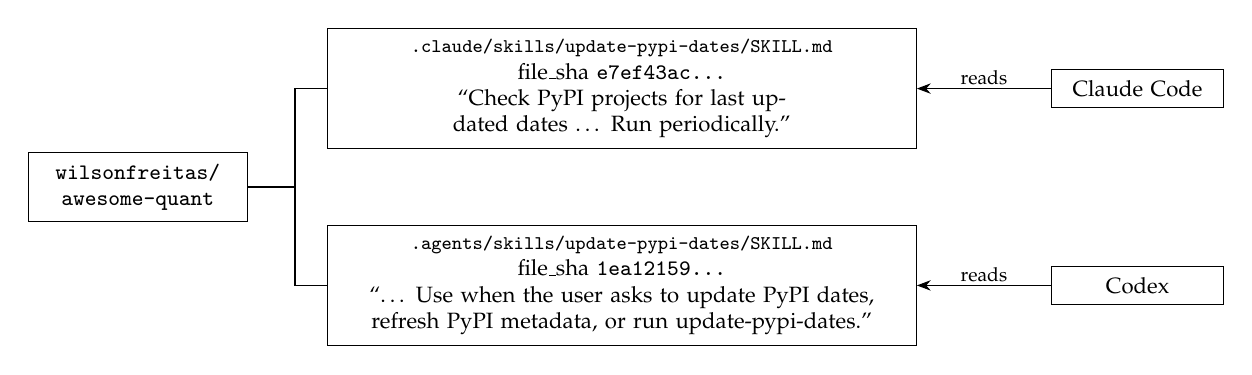
\begin{tikzpicture}
\node[box,text width=2.5cm] (repo) at (0,0) {\texttt{wilsonfreitas/}\\\texttt{awesome-quant}};
\node[box,text width=7.2cm,anchor=west] (c) at (2.4,1.25) {{\scriptsize\texttt{.claude/skills/update-pypi-dates/SKILL.md}}\\ file\_sha \texttt{e7ef43ac\ldots}\\ ``Check PyPI projects for last updated dates \ldots\ Run periodically.''};
\node[box,text width=7.2cm,anchor=west] (a) at (2.4,-1.25) {{\scriptsize\texttt{.agents/skills/update-pypi-dates/SKILL.md}}\\ file\_sha \texttt{1ea12159\ldots}\\ ``\ldots\ Use when the user asks to update PyPI dates, refresh PyPI metadata, or run update-pypi-dates.''};
\node[box,text width=1.9cm,anchor=west] (cc) at (11.6,1.25) {Claude Code};
\node[box,text width=1.9cm,anchor=west] (cx) at (11.6,-1.25) {Codex};
\draw[thin] (repo.east) -- ++(6mm,0) |- (c.west);
\draw[thin] (repo.east) -- ++(6mm,0) |- (a.west);
\draw[arr] (cc.west) -- node[lab,above]{reads} (c.east);
\draw[arr] (cx.west) -- node[lab,above]{reads} (a.east);
\end{tikzpicture}
\caption{A conflicting copy as RQ1 counts it: one skill name, two agent directories, two content hashes, and each product reads only its own copy.}
\label{fig:drift}
\end{figure}

The documentation does not say how the representative copy was chosen, or whether the 24\% of contents with commit
history were picked at random (we assume not). \texttt{canonical} in \texttt{location\_class} looks like it means paths of
the form \texttt{<something>/skills/<name>/SKILL.md}, but we have not confirmed that and are not using the column.

\section{Research questions and related work}

\subsection{Questions}
\begin{itemize}
  \item \textbf{RQ1 (conflicting copies).} How often does a repository give its coding agents different copies of the same
    skill, meaning the same skill name in two agent directories with different content? The unit is the repository, and
    within it the pair of directories. Fields: \texttt{repo\_full\_name}, \texttt{path}, \texttt{name}, \texttt{file\_sha},
    \texttt{description}, and the commit dates.
  \item \textbf{RQ2 (competing skills).} How often do differently named skills in one catalog compete, meaning a realistic
    request could reasonably be answered by either? The unit is the catalog, with estimates reported per repository. Fields:
    name, description and invocation flags of the representative copy, plus catalog size.
  \item \textbf{RQ3 (secondary).} What do skill authors do about this? How often do descriptions refer to another skill, use
    ``do not use for'' wording, or set invocation flags? We had also planned to test whether competition changes what an agent
    does, but another group has now done that at a scale we cannot match (Section 3.3), so that is now an extension if time
    allows.
\end{itemize}

\subsection{Why the questions matter}
The main agent products all pick skills the same way: the model is given a list of names and descriptions and chooses from
it, and none of them check whether two skills mean the same thing
\cite{claudecodeskills2026,codexskills2026,agentskillsspec2026}. Claude Code's documentation says as much: ``If descriptions
are vague or overlap, Claude may load the wrong skill or miss one that would help.'' Same-name skills are handled by a
precedence rule that differs by product (Claude Code prefers a personal skill over a project skill; Codex and VS Code list
both), and the user is never told when the rule has kicked in. A repository that mirrors its skills into several agent
folders can therefore give different agents different instructions as soon as the copies drift, with nothing in the tooling
pointing it out.

From an open-source point of view, skills are a new artifact that gets copied around a great deal: half of all occurrences
in GitSkills are exact copies of a file in another repository, and a tenth of repositories keep parallel copies for several
agents. The problems of copied code are well known (copies drift, a fix lands in one copy and not the others), and we expect
the same here, with the complication that the copy is read by a language model rather than a person who might notice it
looks stale.

\subsection{What related work tells us and what remains open}
The published work is all from the last year or so and mostly experimental: the authors build a skill library and measure
what a model does with it rather than looking at libraries people actually have. Li
\cite{li2026singleagent} added near-synonym competitors to a library and found that one competitor per skill reduced
selection accuracy by 7 to 30\% and two by 17 to 63\%, though the library was synthetic and only two models were tested. Chen
et al.\ \cite{chen2026scaling}, with 15 models and 1{,}141 real skills, found that routing accuracy drops with the logarithm
of library size and that the errors concentrate among similar skills; rewriting the boundaries between similar skills
recovered much of the loss, which bears on our RQ3. Song and Wei \cite{song2026shadowing} report pass rates falling by up to
21\% at 202 skills and attribute this to selection rather than to the longer context. A production team named the same
phenomenon ``skill collision'' \cite{zhou2026collision} and concluded that rewriting cannot fully separate skills whose
intended scopes overlap, which is roughly our definition of competing.

Work on duplication has looked across the ecosystem rather than inside repositories: clone detection over a registry
\cite{zhu2026clones}, name and description matching across a registry \cite{jia2026islands}, and Gao et al.'s finding
\cite{gao2026reuse} that 53\% of reused skills are never modified after adoption (we had first taken that figure to be
58.8\%, which is the share updated at least once).

The paper closest to ours appeared while we were writing this. ``One Skill Too Many'' \cite{oneskilltoomany2026}, by Yan, Xu,
Li, Xu, Liu, Deng and Ma, was posted on October 8, 2026. They built a corpus of 105{,}302 non-fork copies from 20{,}947
repositories (collected July 18, 2026), reconstructed which skills were installed together for 5{,}106 of them, found similar
co-installed pairs with Qwen3 embeddings and an LLM judge (two human raters checked 100 pairs, Krippendorff's $\alpha$ 0.72
to 0.76), and ran 6{,}368 Claude Code sessions. About one in four installed skills has a similar skill beside it, the
installed skill is used 19.9 percentage points less often when a similar one is present, and a guard on the first file read
fixes most of that. They did not look at other agents' directories (their inventory excludes them explicitly) or at drift
between copies. We have read the arXiv HTML version but not the appendices, nor yet the follow-up ``One Skill Takes Over''
\cite{oneskilltakesover2026}.

As far as we can find, nobody has measured drift between mirrored copies across agent directories, which is RQ1. The
prevalence of competing descriptions has now been measured on about 21k repositories with an LLM judge, but not on GitSkills,
which has thirteen times as many, and not with human labels and a sampling design. The earlier work detects overlap with
similarity cut-offs between 0.45 and 0.95 depending on the paper, mostly without checking that the cut-off does what it
claims; in our pilot no cut-off gave even 80\% truly competing pairs, so we use similarity only to decide what to read. Our
own behavioral experiment would mostly repeat the October paper with far less compute, so it is now an ``if time allows.''

\section{Proposed method}

\begin{table}[h]
\centering\small
\begin{tabularx}{\textwidth}{p{2.1cm}p{2.9cm}YY}
\toprule
Question & Unit of analysis & Required fields & Analysis \\
\midrule
RQ1 & Repository; (repository, directory pair); skill name & \texttt{repo\_full\_name}, \texttt{path}, \texttt{name},
  \texttt{file\_sha}, \texttt{description}, commit dates & Exact counts over all repositories; diverged copies classified as
  description changed, body changed, or both; which copy is newer; by which product reads which directories; Wilson
  intervals for every rate \\
\addlinespace
RQ2 & Catalog; estimates per repository & name, description, invocation flags, catalog size; similarity for sampling only &
  Stratified sample of about 750 pairs labeled by two coders; design-based prevalence with repository-clustered intervals;
  by catalog size and relation type; Cohen's $\kappa$ \\
\addlinespace
RQ3 (secondary) & Skill; pair & description text; front-matter flags & Exact counts of cross-references, negative triggers
  and \texttt{disable-model-invocation}; a small routing check if time allows \\
\bottomrule
\end{tabularx}
\caption{How each question maps to a unit, the fields it needs, and the analysis.}
\end{table}

RQ1 and RQ3 are counts over the whole dataset and need no sampling. RQ2 is a human judgment about pairs of skills, so it
needs a sample, an estimator and a reliability check. Figure~\ref{fig:design} shows how the three questions branch off the
same population.

\begin{figure}[h]
\centering
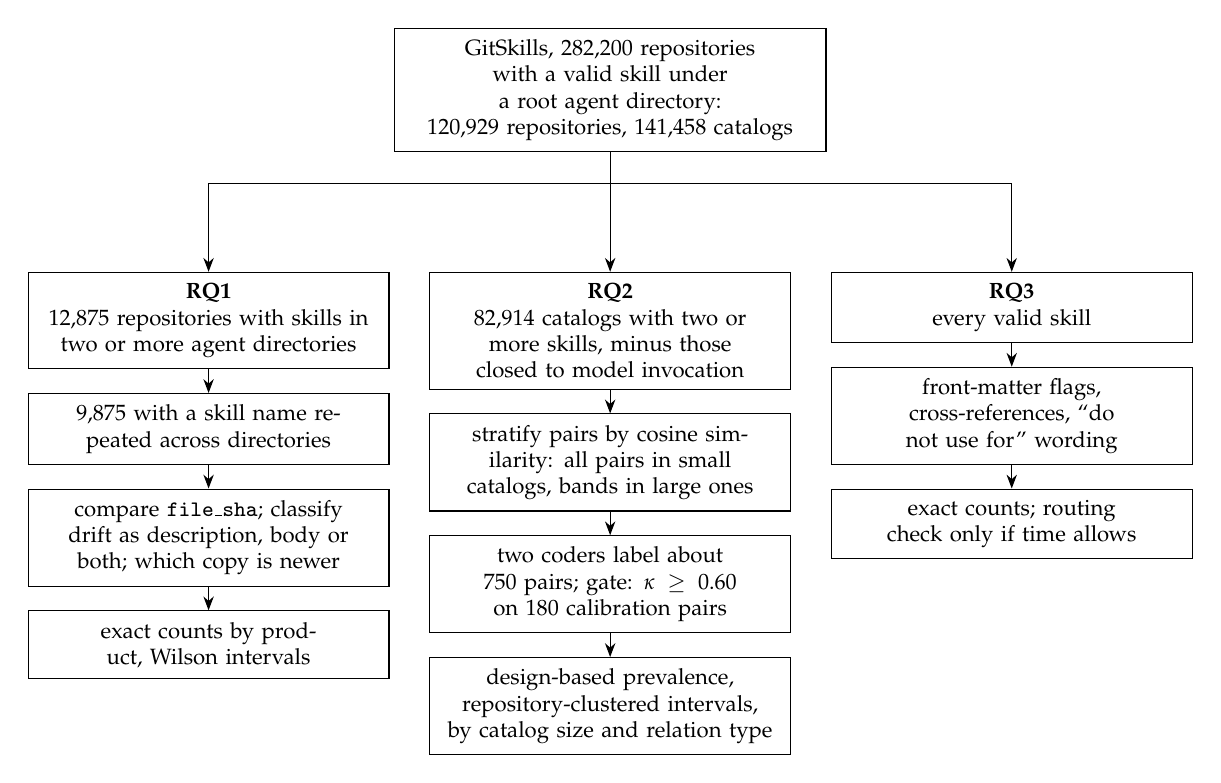
\begin{tikzpicture}[col/.style={box,text width=4.3cm,anchor=north}]
\node[box,text width=5.2cm,anchor=north] (pop) at (0,0) {GitSkills, 282{,}200 repositories\\ with a valid skill under a root agent directory:\\ 120{,}929 repositories, 141{,}458 catalogs};
\node[col] (r1a) at (-5.1,-3.1) {\textbf{RQ1}\\ 12{,}875 repositories with skills in two or more agent directories};
\node[col,below=3mm of r1a] (r1b) {9{,}875 with a skill name repeated across directories};
\node[col,below=3mm of r1b] (r1c) {compare \texttt{file\_sha}; classify drift as description, body or both; which copy is newer};
\node[col,below=3mm of r1c] (r1d) {exact counts by product, Wilson intervals};
\node[col] (r2a) at (0,-3.1) {\textbf{RQ2}\\ 82{,}914 catalogs with two or more skills, minus those closed to model invocation};
\node[col,below=3mm of r2a] (r2b) {stratify pairs by cosine similarity: all pairs in small catalogs, bands in large ones};
\node[col,below=3mm of r2b] (r2c) {two coders label about 750 pairs; gate: $\kappa \ge 0.60$ on 180 calibration pairs};
\node[col,below=3mm of r2c] (r2d) {design-based prevalence, repository-clustered intervals, by catalog size and relation type};
\node[col] (r3a) at (5.1,-3.1) {\textbf{RQ3}\\ every valid skill};
\node[col,below=3mm of r3a] (r3b) {front-matter flags, cross-references, ``do not use for'' wording};
\node[col,below=3mm of r3b] (r3c) {exact counts; routing check only if time allows};
\draw[arr] (pop.south) -- ++(0,-4mm) -| (r1a.north);
\draw[arr] (pop.south) -- (r2a.north);
\draw[arr] (pop.south) -- ++(0,-4mm) -| (r3a.north);
\foreach \a/\b in {r1a/r1b,r1b/r1c,r1c/r1d,r2a/r2b,r2b/r2c,r2c/r2d,r3a/r3b,r3b/r3c} \draw[arr] (\a) -- (\b);
\end{tikzpicture}
\caption{Study design. RQ1 and RQ3 are exact counts; RQ2 is the only sampled estimate and the only one behind a reliability gate.}
\label{fig:design}
\end{figure}

The population is the 120{,}929 repositories with at least one valid skill (a file named exactly \texttt{SKILL.md} whose
front matter parses with a non-empty name and description) under a repository-root agent directory. RQ1 narrows to the
12{,}875 with skills in two or more such directories; RQ2 uses the 82{,}914 catalogs with two or more valid skills, minus
those closed to model invocation (2.45\% of skills set \texttt{disable-model-invocation: true}, and the model never sees
their description). Catalogs whose listing would exceed a product's character budget (4.5\% of multi-skill catalogs at
8{,}000 characters) are flagged, since the product may silently drop descriptions, but kept.

For RQ1 a conflict is the same front-matter name (trimmed and lower-cased) in two directories of one repository with
different \texttt{file\_sha} values, sub-classified by whether the descriptions differ. For RQ2 two skills compete when ``a
realistic request exists for which an agent reading only these two names and descriptions could reasonably pick either.''
The full definition, decision rules and three relation types (D duplicate or variant, S one scope containing the other, O
partial overlap) are in \texttt{docs/codebooks/competing-pairs.md}. The codebook is on its third version, mainly because our
first pilot readers were shown descriptions without the skill names, which turned out to carry much of the signal.

Sampling for RQ2 stratifies on cosine similarity between description embeddings (all-MiniLM-L6-v2). In small catalogs we
read every pair; in large ones we draw pairs from within similarity bands. The estimator is the usual stratified one, with
intervals clustered by repository since one repository can contribute several catalogs. We report prevalence by catalog size,
because the chance of at least one competing pair rises with the number of skills whatever the authors do. RQ1 counts will
be broken down by product: Claude Code reads only \texttt{.claude}, Codex only \texttt{.agents}, while Copilot, Cursor and
OpenCode read several directories at once, so one repository can present a conflict to one product and not another.

For validation, both of us labeled a calibration set of 180 pairs independently. We will compute Cohen's $\kappa$ on
competing versus not competing and go ahead with the main sample only if it reaches 0.60 \cite{landis1977kappa}. Since 29 of
the 180 pairs have a side that is not in English, we had one DeepL translation made and both used it, and will report
$\kappa$ separately for the English and translated subsets. We also had an LLM reader (coder C) label the same pairs from the
codebook alone, for comparison, not adjudication. B versus C gives $\kappa = 0.17$ (95\% interval 0.03 to 0.31); B marked
63\% of pairs as competing and C 39\%, and 61 of the 82 disagreements go the same direction (B competing, C not), which looks
like two readers applying different strictness to ``a realistic request'' rather than disagreeing at random. Coder A's
export came back incomplete and is being redone, so the A versus B number, the one the gate depends on, is not in this
report.

The limitations we know about: repositories hold only project-level skills, so every figure is a lower bound; the product
behavior we rely on is what was documented in July 2026 and could change before the paper is reviewed (Claude Code's listing
rules changed at least twice between February and May 2026, according to its release notes); machine translation flattens
the quoted trigger phrases many descriptions contain; some RQ1 divergence will be deliberate adaptation for one agent; and
the representative copy's commit date understates the age of the content.

\section{Initial data-quality checks}

\subsection{What we have observed}
Front matter fails to parse or lacks a name or description in 10.8\% of occurrences, and those rows are out of both
questions. The front-matter name differs from the folder name in 24.3\% of valid occurrences, so we key on the front-matter
name, which is what the products display. Exact duplicates within one catalog (same name or description) are rare, 0.97\% of
multi-skill catalogs, while copies across directories of the same repository are common (9{,}875 repositories).

Commit history covers 24.4\% of distinct contents and we treat that subset as non-random, so any trend will be stated as
conditional on the skills that have dates. If time allows we will fill in missing dates through the GitHub API; the script
exists and we estimate about a day of polling for the roughly 64{,}500 requests. The latest \texttt{first\_commit\_at} among
representatives is July 23, 2026, after mining ended, so history was fetched a few days after the search; we use July 20 as
the reference date.

Language was a bigger problem than we had planned for. In the calibration set, 29 of 180 pairs (16\%) have a non-English
side: Chinese in 12, Japanese in 8, Spanish and Korean in 3 each, Portuguese, Vietnamese and Norwegian in one each. We handle
it with a single shared machine translation (Section 4) and have not decided what to do if the translated subset disagrees
badly.

While reading pilot pairs we found one e-mail address inside a skill description and removed it from our working files; the
paper will report aggregates only, and row-level files naming repositories stay out of the public repository. One
specification issue affects what coders see: 1.3\% of never-edited skills have descriptions longer than the
1{,}024-character limit in the Agent Skills specification, so we truncate at the product's listing cap before showing text
to a coder.

One problem from the retired-model pilot could recur: a single repository (\texttt{ssrjkk/claude-skills}) contributed
4{,}775 generated skills carrying the same front-matter tag, and until we noticed, it was inflating a dataset-wide
percentage by several points. That is one reason we report at the repository level rather than per skill.

\subsection{Risks still to investigate}
The biggest open question for RQ1 is whether diverged copies differ in substance or only in agent-specific front matter;
the only way to find out is to read diffs, which we have started informally but not on a drawn sample. For RQ2 the risk is
the calibration gate: if the two of us disagree in the same direction, as B and C did, the plan is one round of codebook
revision and a fresh set of pairs, and if that fails we rethink RQ2 rather than keep revising. We have also not looked
at how \texttt{location\_class} and the choice of representative interact with our definition of a library, or whether
\texttt{artifact\_siblings} matters for anything we do; our guess is that it does not.

\section{Work plan and responsibilities}

\begin{table}[h]
\centering\small
\begin{tabularx}{\textwidth}{llY}
\toprule
Date & Milestone & Deliverable \\
\midrule
Oct 22 & Checkpoint 1 & This report; in-class demonstration of the RQ1 query on the Parquet files \\
Oct 23 & Calibration & A versus B $\kappa$ computed and logged; codebook revised if below 0.60; peer feedback exchanged \\
Oct 30 & Data ready & RQ1 counts on all repositories; RQ2 sample drawn and translated; rules logged before computing \\
Nov 3 & Progress report & RQ1 results, calibration result, sampling plan, first figure \\
Nov 13 & Labels done & About 750 pairs labeled by both coders; disagreements resolved \\
Nov 20 & Analysis frozen & All estimates, intervals and figures; replication package drafted \\
Dec 3 & Presentation & In-class talk \\
Dec 9 & Course paper & Full paper in MSR format \\
Dec 18, 23 & MSR deadlines & Abstract; anonymized paper for review (same content) \\
\bottomrule
\end{tabularx}
\caption{Milestones. We plan around the course dates, since the MSR deadlines come later.}
\end{table}

Chris is responsible for the data pipeline in \texttt{src/}, the RQ1 counts, the sampling, the statistics and figures, and
the repository; Smirthya for the related work, the codebook, drafting and editing the paper, and leading the progress report
and the presentation. Both of us label (as coders A and B), resolve disagreements together, and review each other's pull
requests. Our advisor, Igor Steinmacher, is helping with the design, the thresholds, and what is expected at this venue.

RQ2 cannot start until the calibration gate is passed, and the size of the main sample depends on how quickly labeling goes
after that; 180 pairs took each of us a few hours. Translation comes before labeling, and filling in commit dates needs a
token and about a day.

Inter-coder agreement is the thing most likely to go wrong; if it stays low after one revision we report two bounds (pairs
both of us call competing, and pairs either of us does) and have our advisor adjudicate. The October paper also took much of the ground we had planned for RQ2 and RQ3, which is why RQ1 is
now the primary contribution and RQ2 a larger, human-labeled replication; we discussed dropping RQ2 and decided against it,
mainly because the labeling is already under way. Beyond that it is a matter of time; the week between Nov 13 and Nov 20 is
tight.

If RQ2 cannot be made reliable, RQ1 can stand alone as an exact-count study with the author-side part of RQ3 beside it. We
also have a fallback we piloted first, on skills that name AI models their vendors have since retired; it has an objective
measure but a smaller population (23{,}806 repositories name a model at all), and we set it aside when the advisor pointed
us toward conflicting skills.

\section{Peer feedback and response}
The peer-review exchange has not happened yet. Once it has, we will add the feedback we received, the changes we made in
response, and anything we decided not to change, with our reasons.

\bibliographystyle{plain}
\bibliography{references}
\end{document}
